% !TEX encoding = UTF-8 Unicode
% !TEX root = project.tex

\section{Software Implementation}
\label{sec:setup}

\begin{figure*}[ht!]
\centering
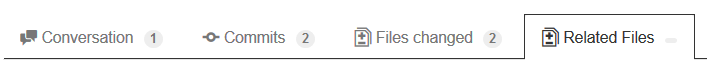
\includegraphics[width=16cm]{NewTabRelatedFiles}
\caption{GitHub pull request page showing the new `Related files' tab}
\label{fig:newTabRelated}
\end{figure*}

\begin{figure*}[ht!]
\centering
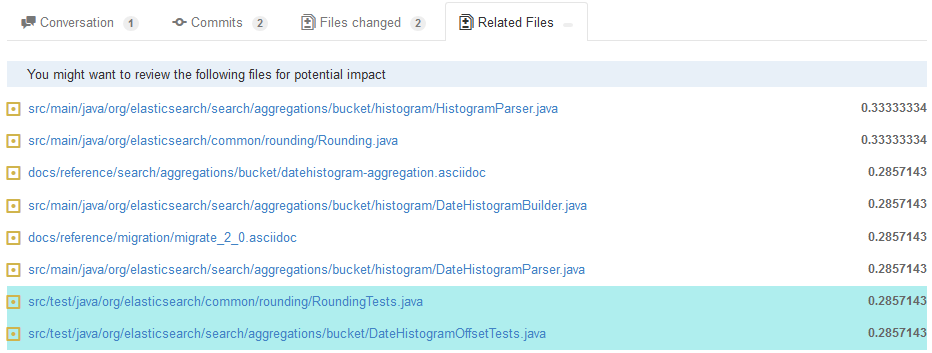
\includegraphics[width=16cm]{RelatedFilesContents}
\caption{`Related files' tab showing files}
\label{fig:relatedFilesContents}
\end{figure*}

\begin{figure*}[ht!]
\centering
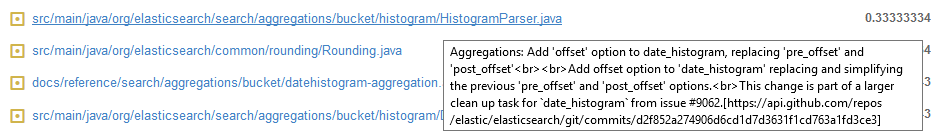
\includegraphics[width=16cm]{MouseOverOfFile}
\caption{Details of the file on performing mouse-over on the hyperlink}
\label{fig:mouseOverOnFile}
\end{figure*}

\begin{figure*}[ht!]
\centering
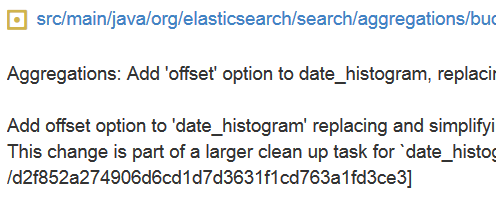
\includegraphics[width=16cm]{ClickOfFileHyperlink}
\caption{Details of the file on clicking on the hyperlink}
\label{fig:clickOnFileHyperlink}
\end{figure*}

\begin{figure}[ht!]
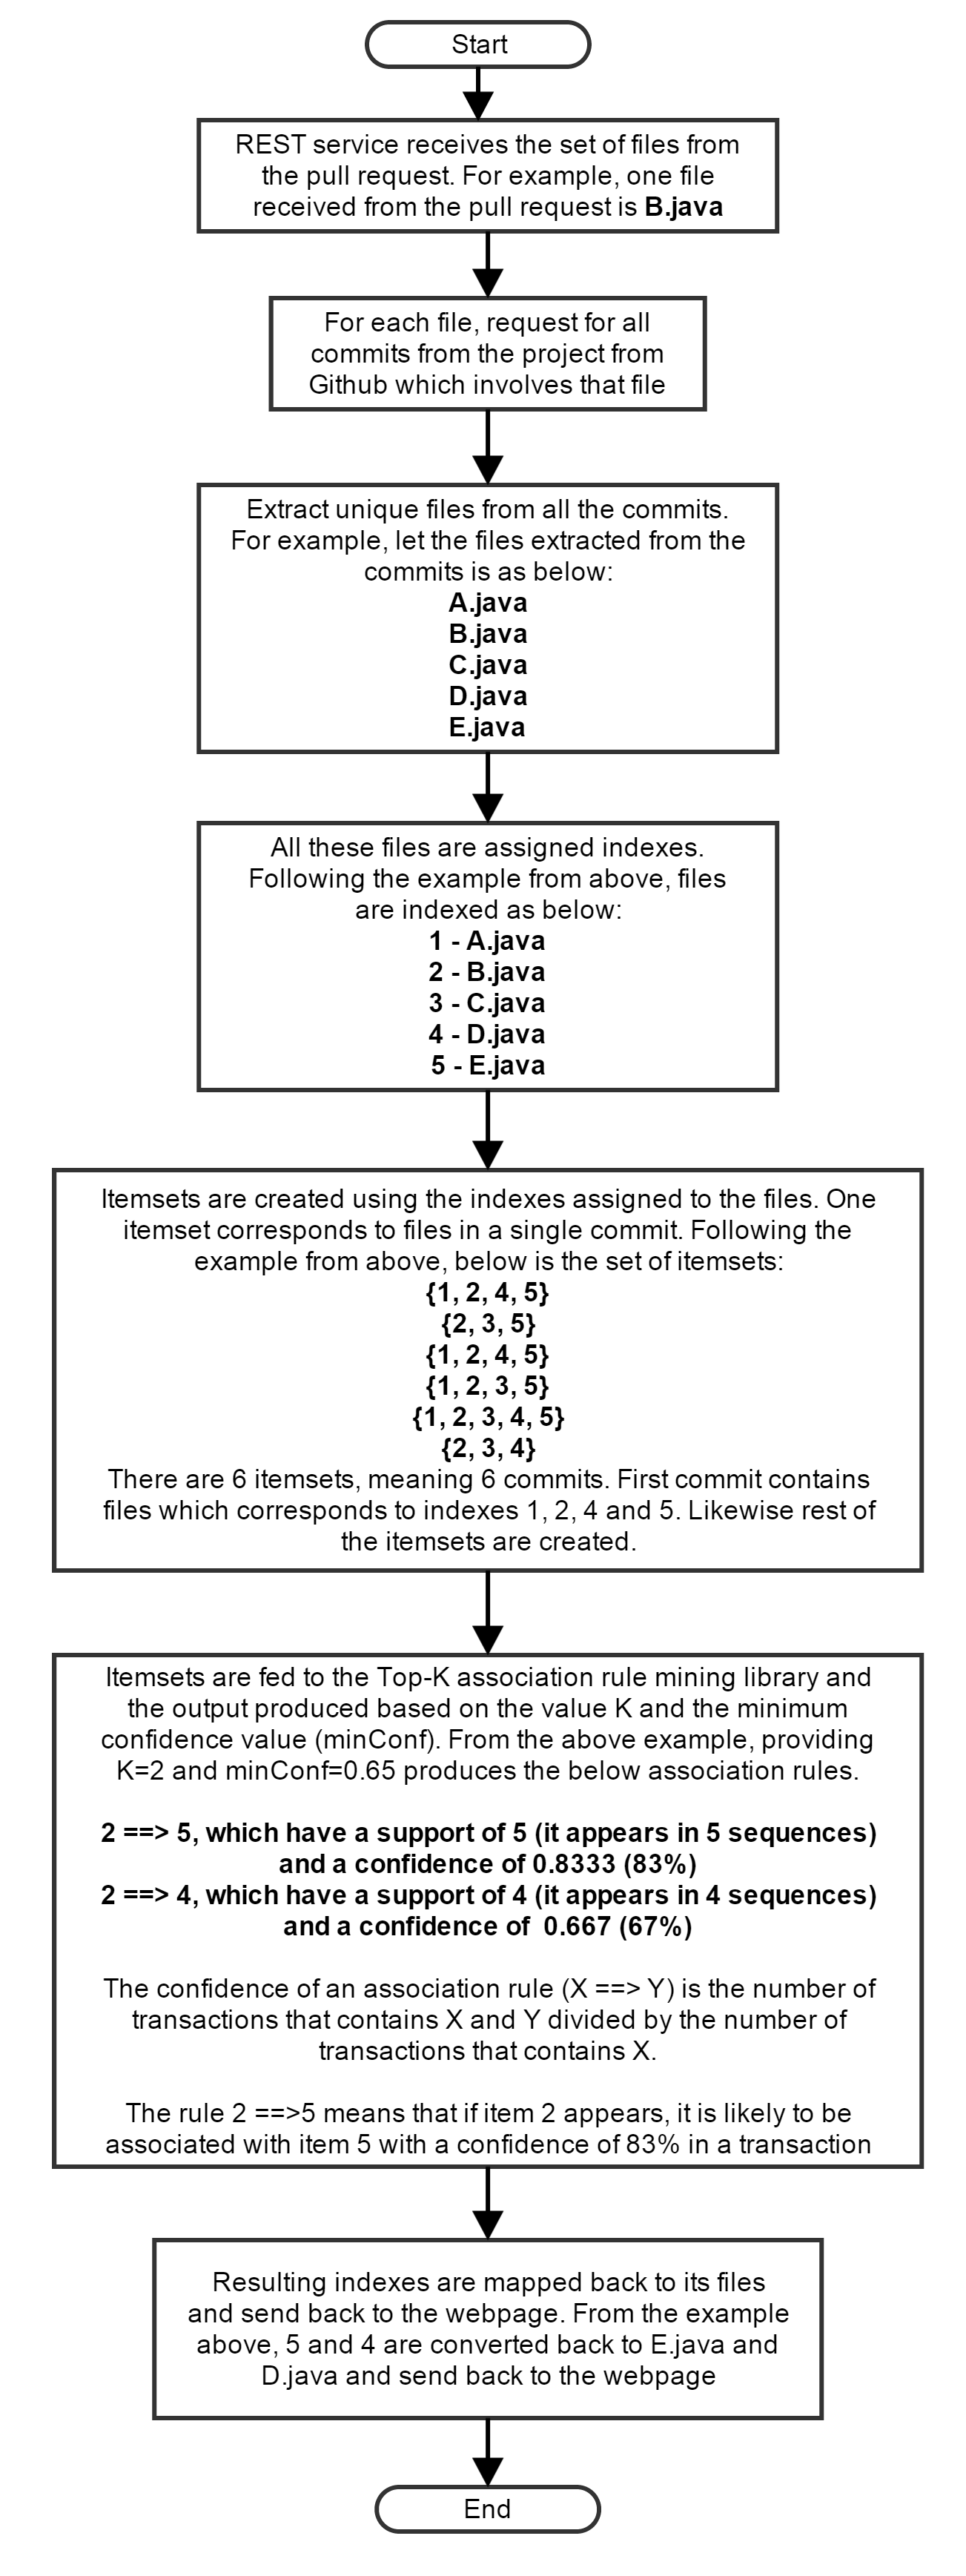
\includegraphics[width=0.5\textwidth]{data_processing_spmf}
\caption{Data processing process flow with example}
\label{fig:data_processing_spmf}
\end{figure}

The software setup was done on a single laptop having an Intel dual-core i5-4210U CPU running at 1.7 GHz with 8 GB RAM, with Windows 8.1 64 bit operating system. In our setup, we created a Javascript user script which was installed on the Firefox browser using GreaseMonkey add-on~\cite{greasemonkey1,greasemonkey2}. When this script is invoked on a GitHub pull request webpage, it adds a new tab named `Related Files' onto the page. Figure~\ref{fig:newTabRelated} shows a screenshot of the webpage showing the new tab. The tab, on opening, sends a REST~\cite{rest} POST~\cite{post_http} request with the all the file names from the pull request in its HTTP message body. The REST service, which is deployed on a Glassfish server~\cite{glassfish}, receives the file names send from the GitHub page. The REST service then makes use of the Top-K association rule mining algorithm~\cite{fournier2012mining} to come up with a list of related file names and is send back to the GitHub page, i.e., from where the request was initiated. The GitHub page will display the results in the 'Related Files' tab. Test files are highlighted in a different color. Details of the algorithm implementation and the data processing are explained in Section~\ref{sec:dataprocessing}.

Figure~\ref{fig:relatedFilesContents} shows the contents of the related files tab populated from the REST service output. A confidence value is shown against each file which is obtained from the association rule mining algorithm.

Figure~\ref{fig:mouseOverOnFile} shows what happens when the mouse is hovered over the hyperlink. It shows the reason why the particular file shows up on the related files tab.

Figure~\ref{fig:clickOnFileHyperlink} shows what happens when the hyperlink is clicked. It is the same reason as above, but user can copy the contents if required.

\subsection{Data processing}
\label{sec:dataprocessing}

We used the Sequential Pattern Mining Framework (SPMF), an open-source data mining library written in Java~\cite{algo_impl}, which consists of an implementation of the Top-K association rule mining algorithm. We used 10 as the value of K, i.e., the library will retrieve at most 10 association rules (we call it the related files) to be discovered. Another input parameter required by the library is the minimum confidence value, which is used to retrieve files which has got at least the provided input confidence value. In our case, we provided 0.1 as the minimum confidence value. We performed some data processing for the purpose of providing data in the required format to the data mining library. First, the list of files is received as input to the REST service. Then, using the GitHub API, all the commits containing these files are retrieved from the particular GitHub project. Then, all these files (initial set of files and the files contained in the commits) are assigned indexes, so that each file can be addressed with a number. For example: Suppose, the filenames are A.java, B.java and C.properties, then they are indexed 1 - A.java, 2 - B.java, 3 - C.properties. A group of itemsets are formed. Each itemset is a series of distinct numbers (which are the indexes assigned to the filenames) which corresponds to the files contained in a particular commit. This group of itemsets are fed to the mining library, which provides the association rules as output. The flow with an example is explained in Figure~\ref{fig:data_processing_spmf}.
